\chapter{Introduction}
\section{Introduction}
Road traffic injuries are a major public health problem and a leading cause of death and injury around
the world. Each year nearly 1.2 million people die as a result of road crashes, and millions more are
injured or disabled. In many low-income and middle-income countries, where motorcycles and bicycles
are an increasingly common means of transport, users of two-wheelers make up a large proportion of
those injured or killed on the roads. Motorcycle and bicycle riders are at an increased risk of being
involved in a crash. This is because they often share the traffic space with fast-moving cars, buses and
trucks, and also because they are less visible. In addition, their lack of physical protection makes them
particularly vulnerable to being injured if they are involved in a collision.\vspace{.5cm}

\paragraph{}In most high-income countries, motorcycle fatalities typically comprise around 5\% to 18\% of overall
traffic fatalities. This proportion reflects the combined effect of several important factors including the
relatively low ownership and use of motorcycles in many developed countries, and the relatively high risk
of these motorcycles being involved in crashes involving fatalities. Typically, these risks are much higher
for motorcycle than for vehicle travel.\vspace{.5cm}

\paragraph{}In low-income and middle-income countries, car ownership and use rates are generally much lower than
in high-income countries. However, the ownership and use of motorcycles and other two-wheelers is
generally relatively high.\vspace{.5cm}

\paragraph{}In India 69\% of the total number of motor vehicles are motorized two-wheelers, considerably higher
than in high-income countries. Reflecting this difference, the levels of motorcycle rider fatalities as a
proportion of those injured on the roads are typically higher in low-income and middle-income countries
than in high-income countries. For instance, 27\% of road deaths in India are among users of motorized
two-wheelers, while this figure is between 70–90\% in Thailand, and about 60\% in Malaysia. In China,
motorcycle ownership between 1987 and 2001 grew rapidly from 23\% to 63\%, with a corresponding increase in the proportion of traffic fatalities sustained by motorcyclists rising from 7.5\% to 19\% over the
same period. However, in other low-income and middle-income countries, a lack of high quality road
safety data means that precise levels of motorcycle rider fatalities are still not known.\vspace{.5cm}

\paragraph{}Traffic accidents in India have been increased every year. As per Section 129 of Motor Vehicles Act, 1988,
every single person riding a two-wheeler is required to wear protective headgear following the standards
of BIS (Bureau of Indian Standards). Also drunken driving under the influence is a criminal offence
according to the Motor Vehicle act 1939, which states that the bike rider will get punishment. Currently
bike riders easily escape from the law. These are the three main issues which motivates us for developing
this project.
\pagebreak

\paragraph{Major reason}for accidental deaths on roads are injuries to the head and neck. In European countries,
head injuries contribute to around 75\% of deaths among motorized two-wheeler users; in some low-income
and middle-income countries head injuries are estimated to account for up to 88\% of such fatalities.In
2017, 48,746 road users on two-wheelers lost their lives in road accidents, which is the single largest
category. Of those who died, 73.8 percent weren’t wearing helmets. The social costs of head injuries for
survivors, their families and communities are high, in part because they frequently require specialized
or long term care. Head injuries also result in much higher medical costs than any other type of injury,
such that these injuries exert a high toll on a country’s health care costs and its economy. Globally,
there is an upward trend in the number and use of motorcycles and bicycles, both for transport and
recreational purposes. Indeed, most of the growth in the number of vehicles on the world’s roads comes
from an increasing use of motorized two-wheelers.
\vspace{.5cm}

\textbf{What is helmet?}
\vspace{.2cm}

A helmet is a form of protective gear worn to protect the head. More specifically, a helmet complements
the skull in protecting the human brain. Ceremonial or symbolic helmets without protective function
are sometimes worn too. Soldiers wear combat helmets, often made from Kevlar or other lightweight
synthetic fibers.
\vspace{.5cm}

\textbf{Why are helmets needed?}
\vspace{.2cm}

considerable rise in the number of motorized two-wheeler vehicles on their roads. This rapid growth in
the use of motorcycles in many lowincome and middle-income countries is already being accompanied by
a considerable increase in the number of head injuries and fatalities that will only continue to increase
if present trends continue unchecked.

\section{Can a helmet protect your head?}
The technical expertise behind the design of high quality helmets is based on an understanding of
what happens to the head in the event of a motorcycle crash. This section describes what happens in
the event of a motorcycle crash, and then explains how a helmet works to reduce this effect.

\subsection{The mechanism of head injuries}
the important anatomical information about the head to note is the following:
\begin{itemize}
	\item The brain is enclosed within a rigid skull.
	\item The brain “sits” on bones that make up the base of the skull.
	\item The spinal cord passes through a hole in the underside of the brain.
	\item Under the skull, adhering to the bones, is a tough tissue called the dura that surrounds the brain.
	\item Between the brain and the dura is a space containing cerebrospinal fluid that protects the brain tissue
	from mechanical shock.
	\item The brain “floats” in the cerebrospinal fluid but it can only move about 1 millimetre in any direction.
	\item The skull is covered by the scalp, which provides some additional protection.
\end{itemize}
\begin{figure}[h]
	\centering
	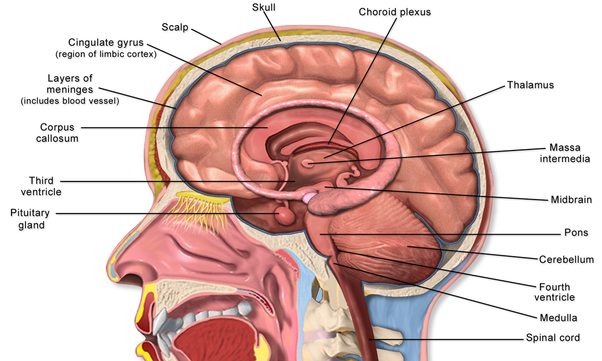
\includegraphics[scale=.35]{main-qimg-fd30ac2527eb37908aa5f1e1c9aa0a27.png}
	\caption{Structure of Head.}
\end{figure}


During a motorcycle or bicycle crash there are two principal mechanisms of injury to the brain: through
direct contact and through acceleration–deceleration. Each mechanism causes different types of injuries.
\vspace{.5cm}

When a motorcycle or bicycle is involved in a collision, the rider is often thrown from the cycle. If the
rider’s head hits an object, such as the ground, the head’s forward motion is stopped, but the brain,
having its own mass, continues to move forward until it strikes the inside of the skull. It then rebounds,
striking the opposite side of the skull. This type of injury can result in anything from a minor head
injury, such as concussion, to a fatal head injury.
\vspace{.5cm}

Head injuries that result from either contact or acceleration–deceleration injuries are themselves divided
into two categories: open or closed head injuries. Most traumatic brain injuries are the result of closed
head injuries – that is, there is no open wound to the brain

\begin{figure}[h]
	\centering
	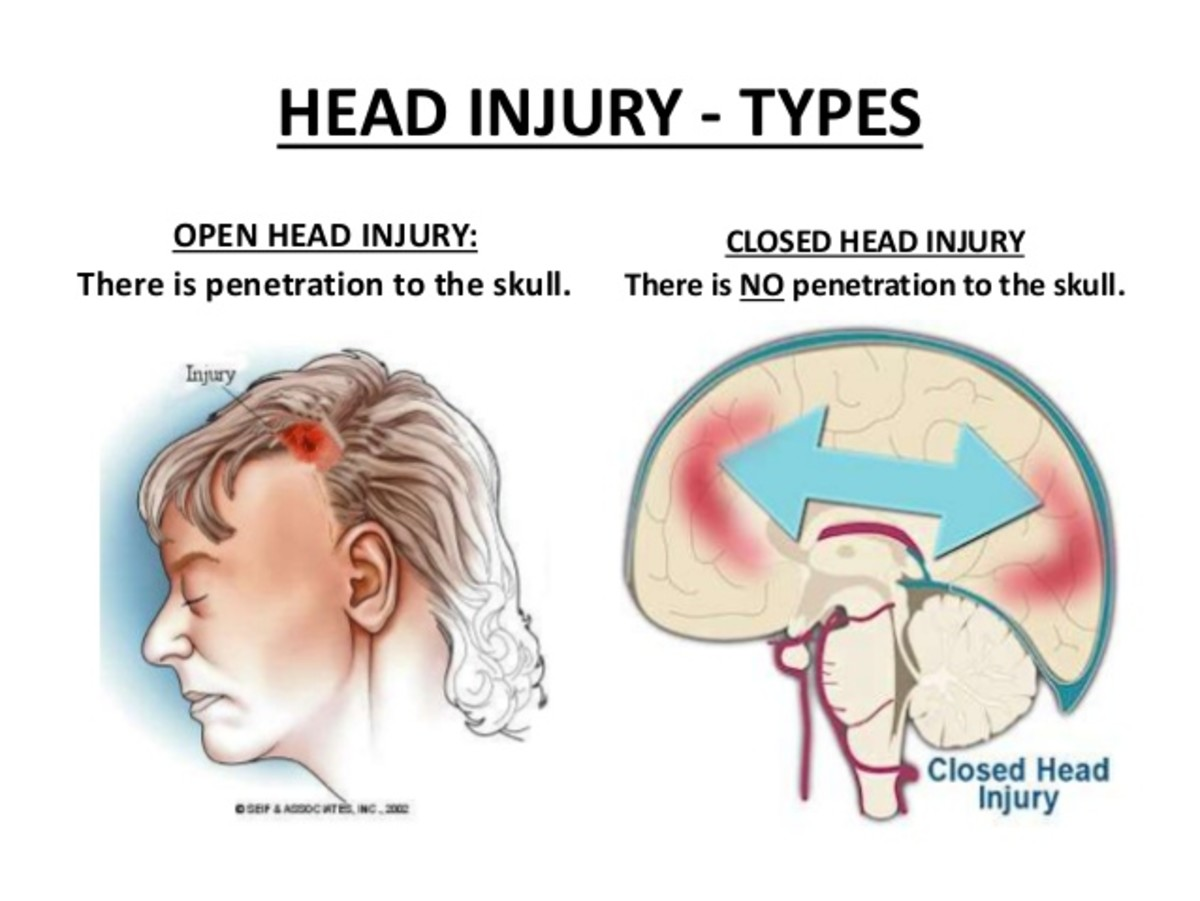
\includegraphics[scale=.8]{learning-to-live-again-with-tbi.jpg}
	\caption{Types of head injuries.}
\end{figure}

Motorcycle riders who do not wear a helmet run a much higher risk of sustaining any of these head and
traumatic brain injuries, or a combination of them. Helmets create an additional layer for the head and
thus protect the wearer from some of the more severe forms of traumatic brain injury

\subsection{How a helmet works}
A helmet aims to reduce the risk of serious head and brain injuries by reducing the impact of a force or
collision to the head.
\begin{itemize}
	\item It reduces the deceleration of the skull, and hence the brain movement, by managing the impact. The
	soft material incorporated in the helmet absorbs some of the impact and therefore the head comes to a
	halt more slowly. This means that the brain does not hit the skull with such great force.
	\item It spreads the forces of the impact over a greater surface area so that they are not concentrated on
	particular areas of the skull.
	\item It prevents direct contact between the skull and the impacting object by acting as a mechanical barrier
	between the head and the object.
\end{itemize}

These three functions are achieved by combining the properties of four basic components of the helmet
that are described below


\begin{figure}[h]
	
	\centering
	
	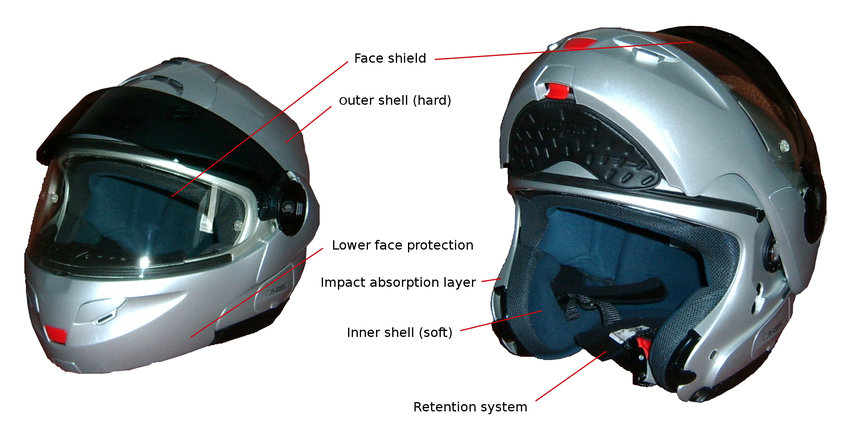
\includegraphics[scale=.7]{Basic-components-of-a-helmet-Photo-in-the-public-domain-adapted-to-remove-background.jpg}
	
	\caption{Components of a helmet.}
	
\end{figure}

\textbf{The shell}\vspace{.2cm}



This is the strong outer surface of the helmet that distributes the impact over a large surface area, and

therefore lessens the force before it reaches the head. Although the shell is tough, it is designed to

compress when it hits anything hard. It provides protection against penetration by small, sharp and

high speed objects and it also protects the padding inside the helmet from abrasions and knocks during

daily use. These requirements mean that the shell must be hard, usually with a smooth exterior finish.\vspace{.4cm}



\textbf{The impact-absorbing liner}\vspace{.2cm}



This is made of a soft, crushable padded material – usually expanded polystyrene, commonly called

“styrofoam”. This dense layer cushions and absorbs the shock as the helmet stops and the head tries to

continue moving.\vspace{.4cm}



\textbf{The comfort padding}\vspace{.2cm}



This is the soft foam-and-cloth layer that sits next to the head. It helps keep the head comfortable and

the helmet fitting snugly.\vspace{.4cm}



\textbf{The retention system, or chin strap}\vspace{.2cm}



This is the mechanism that keeps the helmet on the head in a crash. A strap is connected to each side of

the shell. Chin and neck straps, which are specifically designed to keep the helmet on during an impact,

must be correctly used for the helmet to function as it is designed to.\vspace{.4cm}

\subsection{Motorcycle helmet design}
In addition to meeting the previously described functions and conforming to standards, a helmet needs to be designed to suit the local
weather and traffic conditions. The following are some of the considerations usually
addressed by helmet designers:
\begin{itemize}
	\item Materials used in the construction of a helmet should not degrade over time, or
	through exposure to weather, nor should they be toxic or cause allergic reactions.
	Currently, the plastic materials commonly used are Expanded Poly-Styrene (EPS),
	Acrylonitrile Butadiene Styrene (ABS), Poly Carbon (PC) and Poly Propylene
	(PP). While the material of the helmet shell generally contains PC, PVC, ABS or
	fibre glass, the crushable liner inside the shell is often made out of EPS – a material
	that can absorb shock and impact and is relatively inexpensive. However, helmets
	with EPS liners should be discarded after a crash, and in any case users should
	replace such helmets after 3–5 years of use.
	\item Standards often set the minimum coverage of a helmet (see Module 3). Half-head
	helmets offer minimal coverage. Full-face helmets should ensure that the wearer’s
	peripheral vision and hearing are not compromised.
	\item To ensure that a helmet can absorb the shock of a crash, the crushable liner should
	be between 1.5 cm and 3.0 cm in thickness.
	\vspace{.5cm}
\end{itemize}
In addition to the previously mentioned design issues, there are also various styles of
helmets which afford different protection. The most common types are:\vspace{.2cm}
\begin{itemize}	
	\item\textbf{Full-face helmets}\vspace{.1cm}
	
	A full face helmet covers the entire head, including the base of the skull to the rear. The face and chin are also protected by a section of material which typically also cradles the visor.	These are the most common type of helmet you’ll see in the streets and take their styling (though muted somewhat) from Moto GP helmets. Safety-wise, these are the best helmets you can buy for road riding. 35\% of all crashes show major impact in the chin bar area. In the absence of this protective plastic/carbon/fibreglass, your face takes all that damage.:\vspace{.2cm}
	
	\begin{figure}[h]
		\centering
		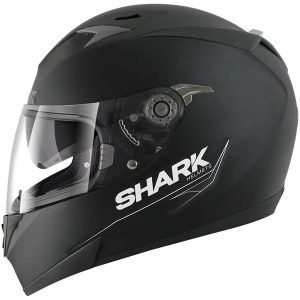
\includegraphics[scale=.35]{shark_s900_special-min-300x300.jpg}
		\caption{Full-face helmet.}
	\end{figure}
	
	\item\textbf{Modular/Flip-Up Helmets} \vspace{.1cm}
	
	Modular helmets attempt to give you the best of both worlds. They include a hinge, allowing the chin bar to be raised and lowered according to the wearer’s needs (even removed in some cases). After full face helmets, these are the next most common type of helmet worn by commuters. When checking the safety rating of a modular helmet, remember that ratings for the helmet in the open and closed position may be stated. If safety ratings only exist for the closed position, the manufacturer doesn’t intend for the helmet to be used while open. In such cases, the ‘open’ feature has been included as a quality of life addition. The convenience of opening the front of your helmet to have a chat or order a coffee is nice, but many people prefer flip ups because they find them quieter. A modular helmet is put on in the open position, meaning the opening at the bottom can be much smaller than a full face face helmet. This results in less air getting into the bottom opening and therefore a quieter experience.
	\begin{figure}[h]
		\centering
		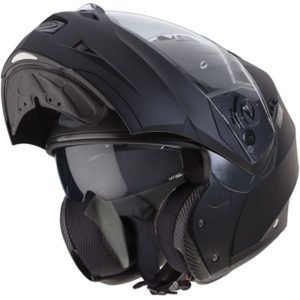
\includegraphics[scale=.35]{helmet_caberg_flip-front_duke_2_matt-black_detail2-300x300.jpg}
		\caption{Modular/Flip-Up Helmet.}
	\end{figure}
	\pagebreak
	
	\item\textbf{Off Road/Motocross}\vspace{.1cm}
	
	Motocross is a physically demanding activity. Riders engaged in this sport need to vent heat much more rapidly than a typical commuter. The chin bar and visor are therefore elongated away from the face, allowing better circulation of air and the use of protective goggles. The visor protects from the sun, but also helps to shield the eyes and face from debris. Paired with a good set of goggles, a quality off-road helmet can offer comparable protection to a full face helmet.
	\begin{figure}[h]
		\centering
		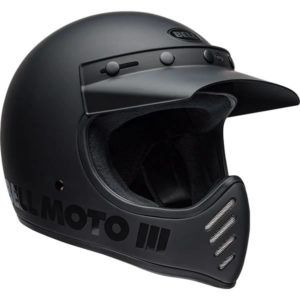
\includegraphics[scale=.35]{bell_helmets_moto-3_blackout-300x300.jpg}
		\caption{Off Road/Motocross.}
	\end{figure}
	
	\item\textbf{Open-face helmets} \vspace{0.1cm}
	
	These helmets, as the name suggests, are open to the front with no chin bar – more common in hotter climates. In tropical conditions, a full face helmet (no matter how good the vents) can be really uncomfortable. Most open face helmets will include a snap-on visor to prevent insects from entering the users eyes. Protection to the head and base of the skull can be equal to that of a full face helmet, but the face is completely unprotected.
	\begin{figure}[h]
		\centering
		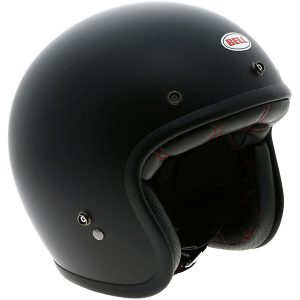
\includegraphics[scale=.35]{word-image-6-300x300.jpeg}
		\caption{Open face helmet.}
	\end{figure}
	
	\item\textbf{Half Helmet/Pudding Basin} \vspace{.1cm}
	
	These look just like they sound. Popular with “bikers”, rockers and street racers, this helmet style has thankfully fallen out of favour in recent years. They can offer some protection from brain injury, but absolutely none to the face. They perform so poorly in both safety tests and real life that many UK manufacturers have stopped producing them.
	\begin{figure}[h]
		\centering
		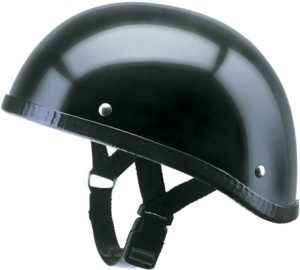
\includegraphics[scale=.35]{RB-100-MATT-SCHWARZ_ml-300x270.jpg}
		\caption{Half Helmet/Pudding Basin.}
	\end{figure}
	
	\item\textbf{Adventure/Dual Sport}\vspace{.1cm}
	
	Adventure/Dual Sport helmets are designed with both on and off-road riding in mind. A boom in adventure riding in the last decade means most major manufacturers offer a few helmets in this category. Common features include a wider face opening for better peripheral vision, enough space to wear goggles, a visor to block the sun/debris and good ventilation. These helmets are equally at home on the road or on a trail. Some high end models have a kind of goggle/visor hybrid that actually works really well. Many offer multiple configurations, removable cold weather features and are suitable for just about any conditions you can throw at them.
	\begin{figure}[h]
		\centering
		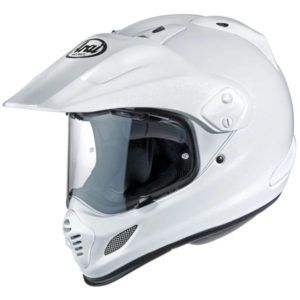
\includegraphics[scale=.35]{arai_tour-x4_diamond-white-300x300.jpg}
		\caption{Adventure/Dual Sport Helmet.}
	\end{figure}
	
	\item\textbf{Smart Helmets} \vspace{.1cm}
	
	This is a pretty new addition to the family, and we haven’t seen any for sale. That said, it’s only a matter of time.The working of smart helmet is very simple, sensors are placed in different places of helmet which are connected to microcontroller board.It is the helmet that works with the help of transmitter and receiver circuit and the microcontroller.
	
	\begin{figure}[h]
		\centering
		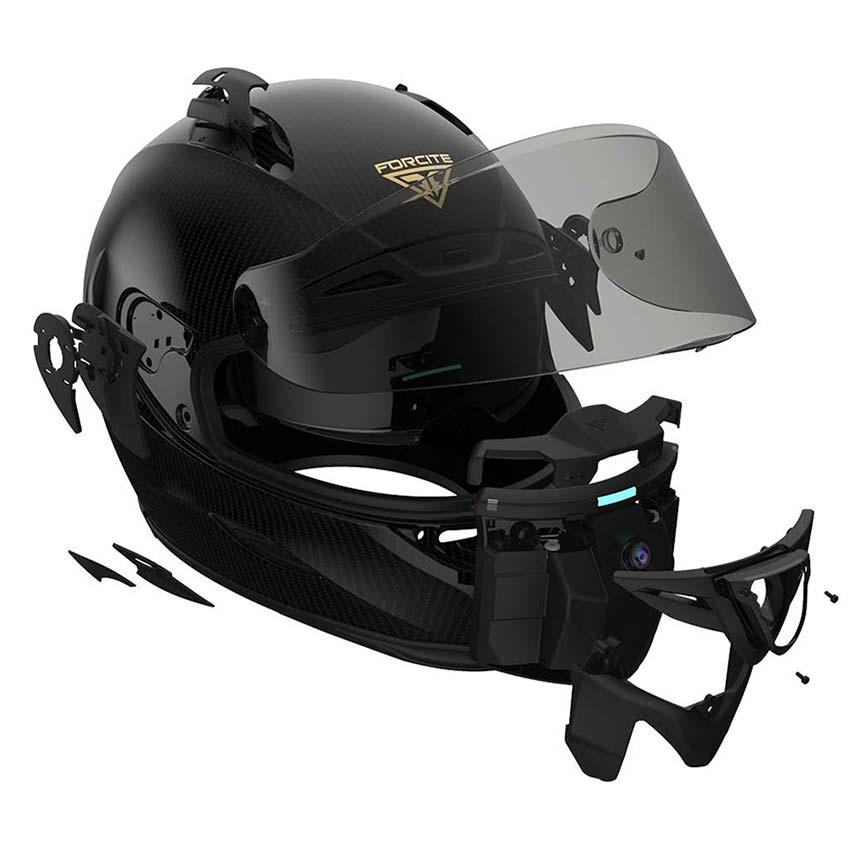
\includegraphics[scale=.15]{forcite-mk1-smart-helmet-australian-2020-09.jpg}
		\caption{Smart Helmet.}
	\end{figure}
\end{itemize} 
\section{Helmet use is effective at reducing head injuries}
Wearing a helmet is the single most effective way of reducing head injuries and fatalities resulting from motorcycle and bicycle crashes. Motorcyclists who do not wear helmets are at a much higher risk of sustaining head injuries and from dying from these injuries. In addition, the disability that results from these head
injuries incurs costs at an individual, family and societal level. There is considerable research that has been conducted on the effects of wearing a helmet on the risk of a head injury as a result of a collision. The results show slightly different effects, depending on the study type, population, situation etc. Consequently it is useful to examine this research collectively – in what is known as a systematic review on the topic of interest. Systematic reviews of studies are a means of objectively examining the evidence for a particular claim (in this case, helmet use in reventing head injury) and combining the results in a way that minimizes any bias. Reviewers conducting such reviews search widely for all the studies on the topic and
include those of a sufficiently high methodological quality. When the data from all the studies included in the review are summarized, the result should provide a more accurate estimate of the effect of the intervention than is possible from individual studies.

\paragraph{}Systematic reviews have been published examining the effectiveness of both motorcycle helmets and bicycle helmets. The review on motorcycle helmets included 53 studies, and summarized the current available evidence on helmets and their impact on mortality, as well as on head, face and neck injuries, following motorcycle crashes. Table 1.1 provides a summary of the main results of this review.  
\begin{table}[h]
	\begin{center}
		\caption{Summary of systematic review of effectiveness of motorcycle helmets.}
		\label{Table 1.1}
		\begin{tabular}{l|l} 
			\textbf{Not wearing a helmet} & \textbf{Wearing a helmet} \\
			\hline
			$\bullet$increases the risk of sustaining a head injury & $\bullet$decreases the likelihood of death by up to 39\%\\
			$\bullet$increases the severity of head injuries & $\bullet$decreases the risk and severity of injuries by about 72\% \\
			
		\end{tabular}
	\end{center}
\end{table}
\pagebreak

The following are the main conclusions of this research:
\begin{itemize}
	\item Motorcycle helmets reduce the risk of mortality and head injury in motorcycle
	riders who crash, although the effect on death may be modified by other factors
	surrounding the crash, such as the speed the motorcyclist was travelling at when
	the crash occurred. Crashes at higher speeds may result in multiple injuries likely
	to cause death, regardless of how well the head is protected. 
	\item There was not enough evidence to determine the effect of motorcycle helmets on
	face or neck injuries, although some studies suggest that helmets have no effect on
	the risk of neck injuries but are protective for face injuries.
	\item There was insufficient evidence to demonstrate whether differences in helmet
	types (full-face versus open-face) confer more or less advantage in injury reduction. Further research should be conducted to determine the effectiveness (and
	cost effectiveness) of different helmet types – especially those used in low-income
	and middle-income countries – on mortality and on head, neck and face injuries.
	\item Increasing motorcycle helmet use in countries where such use has been low is likely
	to dramatically reduce head injury and death. Policy-makers would do well to consider measures to increase helmet use, such as legislation for compulsory helmet
	use and its enforcement, along with community education campaigns.
\end{itemize}


\section{Need Of Project}
Motorcycle safety related to different features of the vehicle such as equipment model, design of the vehicle and as well as operator skill is special for motorcycle rider has towards the motorbikes. But they are the most unsafe road users, without a protective body, even the slightest careless can have serious injuries or may lead to the death of the rider. Not only because of the careless, but the death of the people may occur due to over speed, rash driving, over consumption of alcohol and violation of traffic rules. But the main reason for brain damage and this leads to immediate death, was the absence of helmet on the person. If the rider wears the helmet, 80\% chances for avoiding head injuries and we can save a life from accidents. With the help of new technologies such as IoT, dangerous traffic situations will not occur. And modelling the motorcycles with the sensors, alert system to the rider and surroundings by a sending message, and to make it mandatory for the bike rider to wear a helmet during his/her ride. In a recent survey, every hour 4 people die in road accidents, 70\% due to not wearing a helmet.

\begin{center}
	\section*{Objective}
\end{center}
The main objective of this project is to design a helmet that provides safety to bike riders and to prevent over a drink and drive cases. It detects whether the rider met with an accident if he meets, then it alerts the guardian about the accident and sends SMS.